\documentclass[ignorenonframetext,]{beamer}
\setbeamertemplate{caption}[numbered]
\setbeamertemplate{caption label separator}{: }
\setbeamercolor{caption name}{fg=normal text.fg}
\beamertemplatenavigationsymbolsempty
\usepackage{lmodern}
\usepackage{amssymb,amsmath}
\usepackage{ifxetex,ifluatex}
\usepackage{fixltx2e} % provides \textsubscript
\ifnum 0\ifxetex 1\fi\ifluatex 1\fi=0 % if pdftex
  \usepackage[T1]{fontenc}
  \usepackage[utf8]{inputenc}
\else % if luatex or xelatex
  \ifxetex
    \usepackage{mathspec}
  \else
    \usepackage{fontspec}
  \fi
  \defaultfontfeatures{Ligatures=TeX,Scale=MatchLowercase}
\fi
% use upquote if available, for straight quotes in verbatim environments
\IfFileExists{upquote.sty}{\usepackage{upquote}}{}
% use microtype if available
\IfFileExists{microtype.sty}{%
\usepackage{microtype}
\UseMicrotypeSet[protrusion]{basicmath} % disable protrusion for tt fonts
}{}
\newif\ifbibliography
\hypersetup{
            pdftitle={R in Parallel},
            pdfauthor={Zecca Lehn ( Twitter: @Zecca\_Lehn )},
            pdfborder={0 0 0},
            breaklinks=true}
\urlstyle{same}  % don't use monospace font for urls
\usepackage{graphicx,grffile}
\makeatletter
\def\maxwidth{\ifdim\Gin@nat@width>\linewidth\linewidth\else\Gin@nat@width\fi}
\def\maxheight{\ifdim\Gin@nat@height>\textheight0.8\textheight\else\Gin@nat@height\fi}
\makeatother
% Scale images if necessary, so that they will not overflow the page
% margins by default, and it is still possible to overwrite the defaults
% using explicit options in \includegraphics[width, height, ...]{}
\setkeys{Gin}{width=\maxwidth,height=\maxheight,keepaspectratio}

% Prevent slide breaks in the middle of a paragraph:
\widowpenalties 1 10000
\raggedbottom

\AtBeginPart{
  \let\insertpartnumber\relax
  \let\partname\relax
  \frame{\partpage}
}
\AtBeginSection{
  \ifbibliography
  \else
    \let\insertsectionnumber\relax
    \let\sectionname\relax
    \frame{\sectionpage}
  \fi
}
\AtBeginSubsection{
  \let\insertsubsectionnumber\relax
  \let\subsectionname\relax
  \frame{\subsectionpage}
}

\usepackage[normalem]{ulem}
% avoid problems with \sout in headers with hyperref:
\pdfstringdefDisableCommands{\renewcommand{\sout}{}}
\setlength{\parindent}{0pt}
\setlength{\parskip}{6pt plus 2pt minus 1pt}
\setlength{\emergencystretch}{3em}  % prevent overfull lines
\providecommand{\tightlist}{%
  \setlength{\itemsep}{0pt}\setlength{\parskip}{0pt}}
\setcounter{secnumdepth}{0}

\title{R in Parallel}
\author{Zecca Lehn ( Twitter: @Zecca\_Lehn )}
\date{3/15/2018}

\begin{document}
\frame{\titlepage}

\begin{frame}{Parallelizationalisms}

``I still think in a parallel universe, I became a mathematician.'' Ken
Liu

\begin{block}{What is Parallel Processing?}

\begin{figure}
\centering
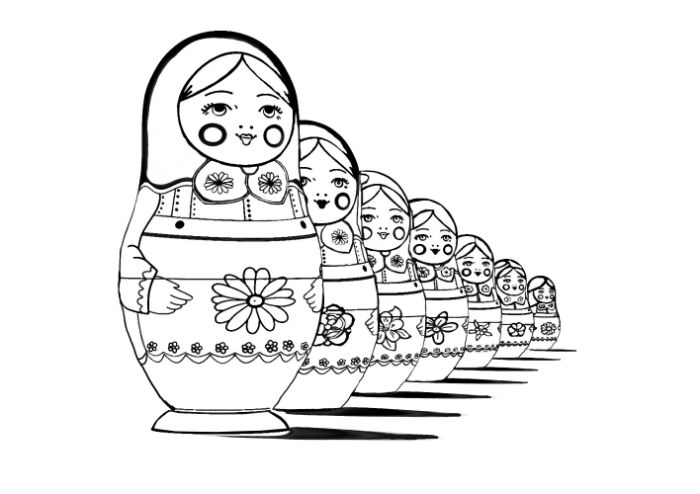
\includegraphics{images/russian-dolls-resized.jpg}
\caption{}
\end{figure}

\end{block}

\begin{block}{``Parallel'' vs. ``Distributed''?}

\begin{figure}
\centering
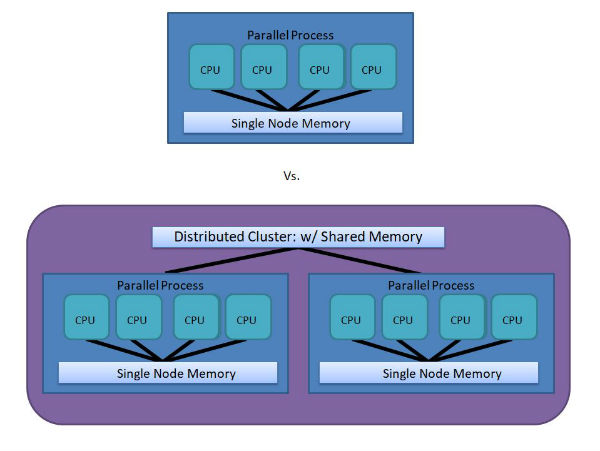
\includegraphics{images/Parallel_vs_Distributed.jpg}
\caption{}
\end{figure}

\end{block}

\begin{block}{Distributed Computing Terms}

\begin{itemize}
\tightlist
\item
  Cluster (`w/Nodes as VMs' distributed)
\item
  Cores (`CPUs' parallelized)
\item
  Thread (`Webpage handler' multithreaded)
\item
  Asyncronous (`Unordered' for speedup and without queue)
\item
  Syncronous (`Ordered' sequences -- DL/apply funcs)
\end{itemize}

\end{block}

\begin{block}{Basic Use Case}

\begin{itemize}
\tightlist
\item
  Speeds up ML training / for-loops
\item
  Reduces cost on per VM basis
\item
  Increases productivity!
\end{itemize}

\end{block}

\begin{block}{From Local VM to Big Data Clusters}

\begin{itemize}
\tightlist
\item
  R/Python (local)
\item
  \sout{Hadoop (Mahout)}
\item
  Spark (PySpark/SparklyR/Spark ML)
\item
  GPUs and TPUs (Tensorflow/Keras/PyTorch)
\end{itemize}

\end{block}

\end{frame}

\begin{frame}{Live Examples in R\ldots{}}

\end{frame}

\begin{frame}{Questions?}

\end{frame}

\end{document}
